\begin{lstlisting}
习题2.5第4题

习题2.6第1,3,7,11,13,15题
\end{lstlisting}
\begin{exercise}
\begin{figure}[H]
\centering
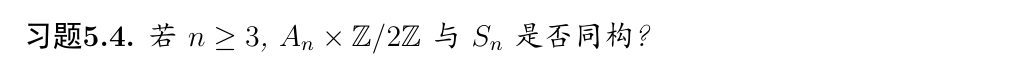
\includegraphics[width=\textwidth]{1-hw6-2025041815.png}
% \caption{}
\label{}
\end{figure}
\end{exercise}
\begin{definition}[product of two groups]
The \textbf{(direct) product} of two groups $(G, *)$ and $(H, \circ)$ is the group $G \times H$ whose underlying set is the Cartesian product of $G$ and $H$, and whose group operation is defined componentwise:
\[
\left(g_1, h_1\right) \cdot\left(g_2, h_2\right)=\left(g_1 * g_2, h_1 \circ h_2\right)
\]for all $g_1, g_2 \in G$ and $h_1, h_2 \in H$.
\end{definition}
\begin{proof}
$A_n\times \mathbb{Z}/2\mathbb{Z}\centernot{\cong}S_n$, because $A_n\times \mathbb{Z}/2\mathbb{Z}$ has nontrivial center
\[
Z(A_n\times \mathbb{Z}/2\mathbb{Z})=(e,\mathbb{Z}/2\mathbb{Z})
\]
But $Z(S_n)$ is trivial.
\end{proof}

\begin{exercise}
\begin{figure}[H]
\centering
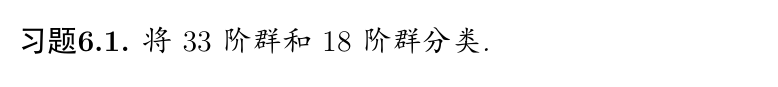
\includegraphics[width=\textwidth]{2-hw6-2025041815.png}
% \caption{}
\label{}
\end{figure}
\end{exercise}
\begin{figure}[H]
\centering
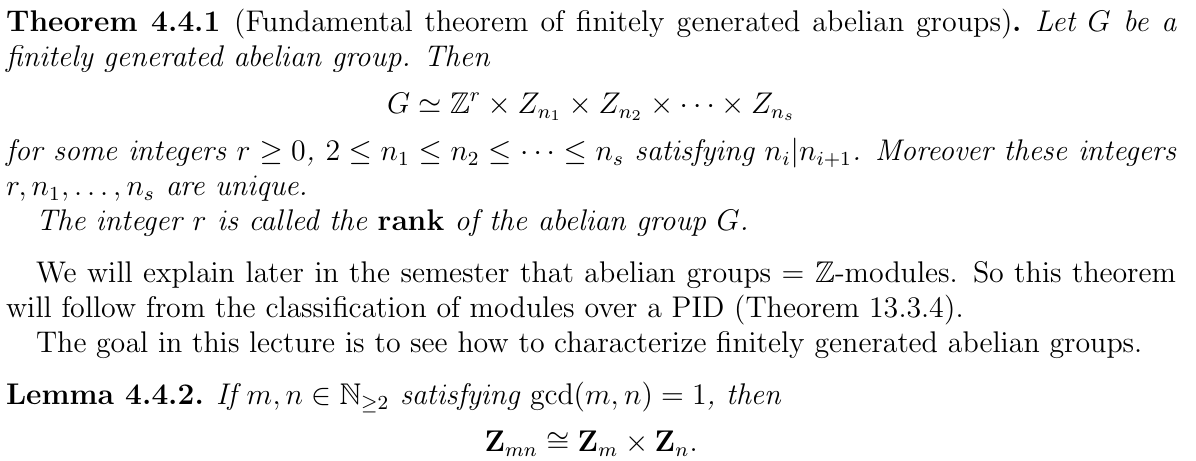
\includegraphics[width=\textwidth]{1-hw6-2025041818.png}
% \caption{}
\label{}
\end{figure}
(1) For $\lvert G \rvert=33=3\times11$, by Sylow III theorem, $n_3=1,n_{11}=1$. Thus $G$ has unique Sylow 3-subgroup $P$ and Sylow 11-subgroup $Q$, which are normal in $G$. For any $p\in P, q\in Q$, we have $pq=qp$, since $pqp^{-1}q^{-1}\in P\cap Q=\{ e \}$. $PQ$ is a group of order 33, since $(p_1q_1)(p_2q_2)^{-1}=(p_1p_2^{-1})(q_1q_2 ^{-1})\in PQ$ for any $p_1, p_2\in P, q_1, q_2\in Q$. Since $PQ\subseteq G$, $\lvert PQ \rvert=33=\lvert G \rvert$, we have $G=PQ$. Therefore $G$ is an abelian group of 33 order. (Moreover, $G$ is cyclic since $P$, $Q$ are cyclic.) By fundamental theorem of finitely generated abelian groups,
\[
G\cong \mathbb{Z}_{3}\oplus  \mathbb{Z}_{11}  =\mathbb{Z}_{3}\times \mathbb{Z}_{11} \cong \mathbb{Z}_{33}
\]
\begin{remark}
The \textbf{direct product} and \textbf{direct sum} construct new groups from a collection of groups.
For a finite number of groups $G_1, G_2, \dots, G_n$, the direct product $G_1 \times G_2 \times \dots \times G_n$ consists of tuples $(g_1, g_2, \dots, g_n)$ where $g_i \in G_i$, with component-wise operation. The direct sum $G_1 \oplus G_2 \oplus \dots \oplus G_n$ is the same as the direct product in this case.
For an infinite collection of groups $\{G_i\}_{i \in I}$, the direct product $\prod_{i \in I} G_i$ consists of all tuples $(g_i)_{i \in I}$ where $g_i \in G_i$. The direct sum $\bigoplus_{i \in I} G_i$ is a subgroup of the direct product, containing only tuples $(g_i)_{i \in I}$ where finitely many $g_i$ are not the identity element in their respective groups $G_i$.
For example, with $G_i = \mathbb{Z}_2 = \{0, 1\}$, the direct product $\prod_{i=1}^{\infty} \mathbb{Z}_2$ can have elements like $(1, 1, 1, 1, 1, \dots)$, while the direct sum $\bigoplus_{i=1}^{\infty} \mathbb{Z}_2$ requires elements with finitely many 1s, such as $(1, 0, 1, 0, 0, 1, 0, 0, \dots)$.
\end{remark}
(2) For $\lvert G \rvert=18=2\times3^{2}$, by Sylow III theorem, $n_3=1$, $n_2\in \{ 1,3,9 \}$.

Let $H$ be the Sylow 3-subgroup of $G$, then it's normal in $G$ (by Sylow ii theorem), with order 9. Pick a Sylow 2-subgroup $K$ of $G$. Since $H\lhd G$, $\lvert K \rvert=2$, $HK$ is a subgroup of $G$ of order $\lvert H \rvert \lvert K \rvert/\lvert H\cap K \rvert=18$, so $G=HK$ and the recognition theorem for semidirect products tells us $G$ is isomorphic to a semidirect product $H\rtimes_{\varphi}K$. The group $H$ is isomorphic to $\mathbb{Z}_{9}$ or $\mathbb{Z}_{3}\times \mathbb{Z}_{3}$. The group $K$ is isomorphic to $\mathbb{Z}_{2}$. Then we are going to classify all semidirect products $\mathbb{Z}_{9}\rtimes \mathbb{Z}_{2}$ and $(\mathbb{Z}_{3}\times \mathbb{Z}_{3})\rtimes \mathbb{Z}_{2}$.

To classify $\mathbb{Z}_{9}\rtimes \mathbb{Z}_{2}$, let $\varphi:\mathbb{Z}_{2}\to(\mathbb{Z}_{9})^{\times}$ be a homomorphism. It is determined by $\varphi(1)$, which is a solution of $a^{2}\equiv1\ \mathrm{mod}\ 9$. By listing all the conditions, $\varphi (1)\equiv 1,-1\ \mathrm{mod}\ 9$. When $\varphi(1)=1$, the homomorphism is trivial and $G\cong\mathbb{Z}_{9}\times \mathbb{Z}_{2}\cong\mathbb{Z}_{18}$. When $\varphi(1)=-1$, we get a semidirect product
\[
\mathbb{Z}_{9}\rtimes \mathbb{Z}_{2}
\]
by
\[
(a,b)(c,d)=(a+\varphi_{b}(c),b+d)=(a+(-1)^{b}c,b+d)
\]
It is isomorphic to $D_{18}$, with an isomorphism
\[
f:\mathbb{Z}_{9}\rtimes_{\varphi}\mathbb{Z}_{2}\to D_{18}= \left< r,s \right>
\]
being given by $f(a,b)=r^{a}s^{b}$. It's clearly a homomorphism. Check the relationships:
\[
r^{9}=f(9,0)=(0,0)\qquad s^2=f(0,2)=(0,0)
\]
\[
rsr=f(1,1)\cdot f(1,0)=f((1,1)(1,0))=f(1+(-1)^{1}\cdot1,1+0)=f(0,1)=s
\]
Thus $f$ is an isomorphism.

To classify $(\mathbb{Z}_{3}\times \mathbb{Z}_{3})\rtimes \mathbb{Z}_{2}$, let $\varphi:\mathbb{Z}_{2}\to(\mathbb{Z}_{3}\times \mathbb{Z}_{3})^{\times}$ be a homomorphism. It is determined by $\varphi(1)$, which is a pair of solution of $a^2\equiv1\ \mathrm{mod}\ 3$. The solutions are $\varphi(1)=(1,1),(1,-1),(-1,1),(-1,-1)$. When $\varphi(1)=(1,1 )$, the homomorphism is trivial, then $G\cong \mathbb{Z}_{3}\times \mathbb{Z}_{3}\times \mathbb{Z}_{2}\cong \mathbb{Z}_{6}\times \mathbb{Z}_{3}$. When $\varphi(1)=(1,-1)$, we get a semidirect product
\[
(\mathbb{Z}_{3}\times \mathbb{Z}_{3}  )\rtimes \mathbb{Z}_{2}
\]
by
\[
(a,b,c)(d,e,f)=((a,b)+\varphi _{c}(d,e),c+f)=(a+d,b+(-1)^{c}e,c+f)
\]
It is isomorphic to $\mathbb{Z}_{3}\times S_3$, with an isomorphism
\[
f:(\mathbb{Z}_{3}\times \mathbb{Z}_{3}  )\rtimes \mathbb{Z}_{2}\to \mathbb{Z}_{3}\times S_3=\mathbb{Z}_{3}\times  \left< (1\ 2),(1\ 3) \right>
\]
being given by $f(a,b,c)=(a,(1\ 2\ 3)^{b}(1\ 2)^{c})$. Similarly, when $\varphi(1)=(-1,1)$, $G$ is isomorphic to $\mathbb{Z}\times S_3$.

When $\varphi(1)=(-1,-1)$, we get a semidirect product
\[
(\mathbb{Z}_{3}\times \mathbb{Z}_{3}  )\rtimes \mathbb{Z}_{2}
\]
by
\[
(a,b,c)(d,e,f)=((a,b)+\varphi _{c}(d,e),c+f)=(a+(-1)^{c}d,b+(-1)^{c}e,c+f)
\]
There are 5 different groups with order 18:

\begin{itemize}
	\item $\mathbb{Z}_{18}$
	\item $\mathbb{Z}_{6}\times \mathbb{Z}_{3}$
	\item $\mathbb{Z}_{3}\times S_3$
	\item $D_{18}$
	\item $(\mathbb{Z}_{3}\times \mathbb{Z}_{3})\rtimes \mathbb{Z}_{2}$, by $(a,b,c)(d,e,f)=(a+(-1)^{c}d,b+(-1)^{c}e,c+f)$.
\end{itemize}

\begin{exercise}
\begin{figure}[H]
\centering
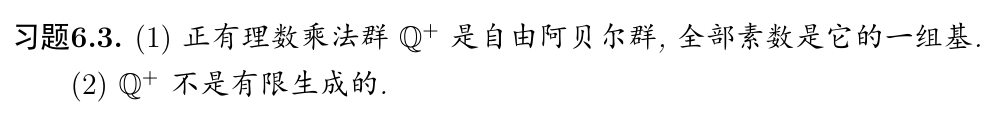
\includegraphics[width=\textwidth]{hw6-2025041816.png}
% \caption{}
\label{}
\end{figure}
\end{exercise}
\begin{definition}[自由阿贝尔群的一组基]
设$G$是一个自由阿贝尔群。$G$的一组\textbf{基}是一个子集$B \subset G$, 满足
	\begin{enumerate}
		\item $B$是$G$的生成集,即$G = \langle B \rangle$。
		\item $B$是线性无关的,即如果对于$b_1, \ldots, b_n \in B$和$z_1, \ldots, z_n \in \mathbb{Z}$, 使得
\[
z_1 b_1 + \cdots + z_n b_n = 0,
\]那么$z_1 = \cdots = z_n = 0$。
	\end{enumerate}
\end{definition}
(1) 记全体素数集合为 $\mathcal{P}$,那么 $\mathbb{Q}^{+}=\mathbb{Z}(\mathcal{P})$,这是因为任意 $x\in \mathbb{Q}^{+}$ 都存在素因子分解
\[
x=p_1^{s_1}\dots p_{r}^{s_{r}}\qquad \text{其中 }s_1,\dots,s_{r}\in \mathbb{Z}
\]
所以 $\mathbb{Q}^{+}\subseteq \mathbb{Z}(\mathcal{P})$,同时由于 $\mathcal{P}\subseteq \mathbb{Q}^{+}$,所以 $\mathbb{Z}(\mathcal{P})\subseteq \mathbb{Q}^{+}$,因此 $\mathbb{Z}(\mathcal{P})=\mathbb{Q}^{+}$.

\begin{figure}[H]
\centering
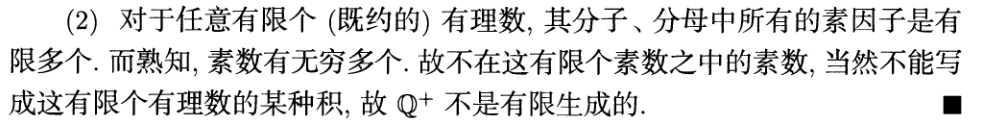
\includegraphics[width=\textwidth]{hw6-2025041822.png}
% \caption{}
\label{}
\end{figure}

\begin{exercise}
\begin{figure}[H]
\centering
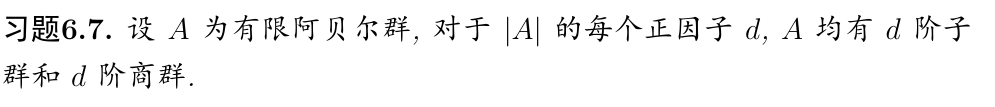
\includegraphics[width=\textwidth]{1-hw6-2025041816.png}
% \caption{}
\label{}
\end{figure}
\end{exercise}
\begin{figure}[H]
\centering
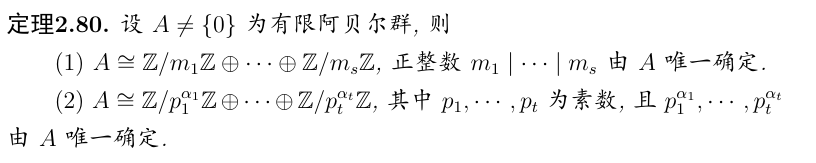
\includegraphics[width=\textwidth]{2-hw6-2025041822.png}
% \caption{}
\label{}
\end{figure}

\begin{figure}[H]
\centering
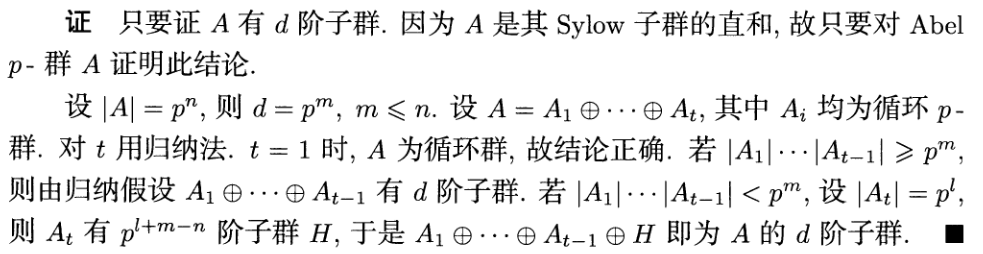
\includegraphics[width=\textwidth]{1-hw6-2025041822.png}
% \caption{}
\label{}
\end{figure}

\begin{exercise}
\begin{figure}[H]
\centering
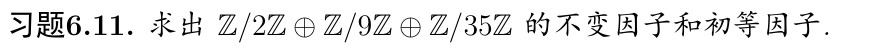
\includegraphics[width=\textwidth]{2-hw6-2025041816.png}
% \caption{}
\label{}
\end{figure}
\end{exercise}
\[
\mathbf{Z}_{2}\times \mathbf{Z}_{9}\times \mathbf{Z_{35}}\cong \mathbf{Z}_{2}\times \mathbf{Z}_{9}\times \mathbf{Z}_{5}\times \mathbf{Z}_{7}\cong \mathbf{Z}_{630}
\]
不变因子为 $\{ 630 \}$,初等因子为 $\{ 2,5,7,9 \}$.

\begin{exercise}
\begin{figure}[H]
\centering
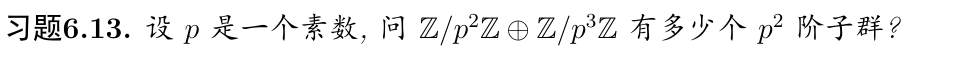
\includegraphics[width=\textwidth]{3-hw6-2025041816.png}
% \caption{}
\label{}
\end{figure}
\end{exercise}
\begin{proof}
\[
\mathbb{Z}_{p^2}\oplus \mathbb{Z}_{p^3}\cong \mathbb{Z}_{p^2}\times \mathbb{Z}_{p^3}
\]
The only $p^2$ -subgroup of $\mathbb{Z}_{p^2}$ is itself. Since $\mathbb{Z}_{p^3}$ is cyclic, the unique $p^2$ -subgroup of $\mathbb{Z}_{p^3}$ is $\left< p \right>$. List all the $p^2$ subgroups.
\[
(\mathbb{Z}_{p^2},\left< p \right> ),(\mathbb{Z}_{p^2},\left< p^2 \right> ),(\mathbb{Z}_{p^2},0),(\left< p \right> ,\left< p \right> ),(0,\left< p \right> )
\]
Thus $\mathbb{Z}_{p^2}\oplus \mathbb{Z}_{p^3}$ has 5 $p^2$ -subgroups.

\end{proof}

\begin{exercise}
\begin{figure}[H]
\centering
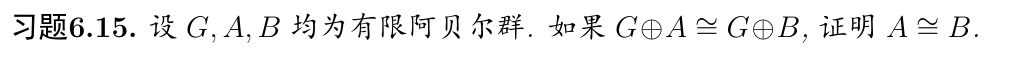
\includegraphics[width=\textwidth]{4-hw6-2025041816.png}
% \caption{}
\label{}
\end{figure}
\end{exercise}
\begin{proof}
Since $G,A,B$ are finite abel groups,
\[
G\times A\cong G\oplus A\cong G\oplus B\cong G\times B
\]
There is an isomorphism $\phi$ between $G\times A$ and $G\times B$. Restrict $\phi$ to the second component by left composing $\pi_2$, then $\pi_2\circ \phi$ is an isomorphism between $A$ and $B$. Thus
\[
A\cong B
\]
\end{proof}
